% =============================================================================
\section{Phase noise}
% =============================================================================

Another important characteristic of a \abbrev{bec} interferometry experiment is the phase noise, which is connected with the visibility.
We will discuss it based on the same experiment~\cite{Egorov2011,Egorov2012} as in the previous section.

While in the simulation we can measure the visibility~\eqnref{bec-noise:visibility:visibility} simply by calculating a second-order moment, experimentalists do not have the luxury of knowing the wavefunctions of the components.
Instead, multiple runs of the Ramsey sequence with the same evolution time are performed, with the second $\pi/2$-pulse having a different phase lag $\phi$ each time.
The quantity that can be measured in the experiment is the normalized atom difference
\begin{eqn}
    P_z = \frac{N_2^\prime - N_1^\prime}{N_1^\prime + N_2^\prime},
\end{eqn}
where $N_1^\prime$ and $N_2^\prime$ are populations of the components obtained by imaging after the second $\pi/2$-pulse.
Using the rotation matrix~\eqnref{bec-noise:mean-field:rotation-matrix} it can be shown that $P_z$ can be expressed in terms of wave operators before the second $\pi/2$-pulse as
\begin{eqn}
    P_z(\phi)
    = - \frac{2}{N_1 + N_2} \Imag \left(
        e^{-i\phi} \int \langle \Psiop_1^\dagger \Psi_2 \rangle \upd\xvec
        \right).
\end{eqn}
One can notice that the integral of the second order moment in this expression is the same as in~\eqnref{bec-noise:visibility:visibility}, and is also normalized on the total population.
Therefore if we vary $\phi$ in the experiment, the resulting $P_z(\phi)$ can be fit with a sine function, and its maximum will give us the visibility $\mathcal{V}$.

\begin{figure}
    \centerline{%
    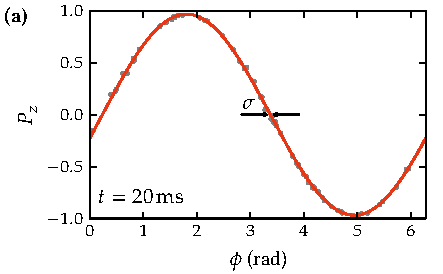
\includegraphics{figures_generated/bec_noise/illustration_noise_20ms.pdf}%
    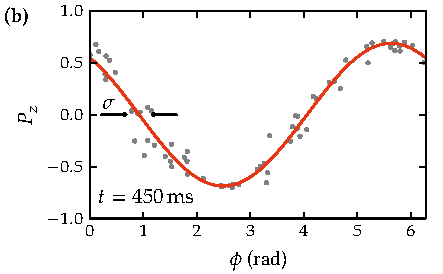
\includegraphics{figures_generated/bec_noise/illustration_noise_450ms.pdf}}

    \caption{Phase noise in the experimental measurement of the visibility.
    Black dots illustrate }

    \label{fig:bec-noise:phase-noise:illustration}
\end{figure}

In practice, naturally, the measurement of $P_z$ is affected by various sources of technical noise.
As a result, the measured points are displaced in phase as compared to the ideal curve, and the width of this displacement $\omega$ is called the phase noise.
This is illustrated in~\figref{bec-noise:phase-noise:illustration} (the ``experimental'' points are taken from different simulation paths in the truncated Wigner simulation of the Ramsey sequence from the previous section).

In the experiment in question three such sources were identified.
First, the length of $\pi/2$-pulses varied throughout the exeprimental runs with an estimated standard deviation of $0.02\un{rad}$.
The phase lag $\phi$ also

\begin{figure}
    \centerline{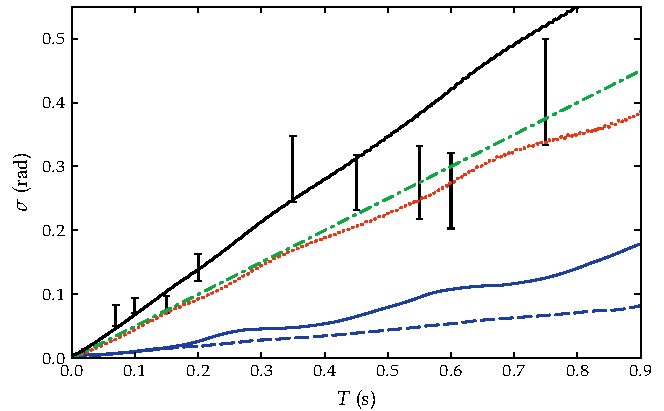
\includegraphics{figures_generated/bec_noise/ramsey_noise.pdf}}

    \caption{Comparison of experimental and numerically simulated interferometric contrast in the Ramsey sequence.
    Plotted are the results obtained with the Wigner method (blue dashed line), Wigner method with the addition of the coupler noise (blue solid line), the noise introduced by the MW frequency instability (green dash-dotted line), the noise introduced by the imaging (red dotted line), and the combination of technical and quantum noises (black solid line), along with the experimental points (black bars).}

    \label{fig:bec-noise:phase-noise:ramsey-phnoise}
\end{figure}

\begin{figure}
    \centerline{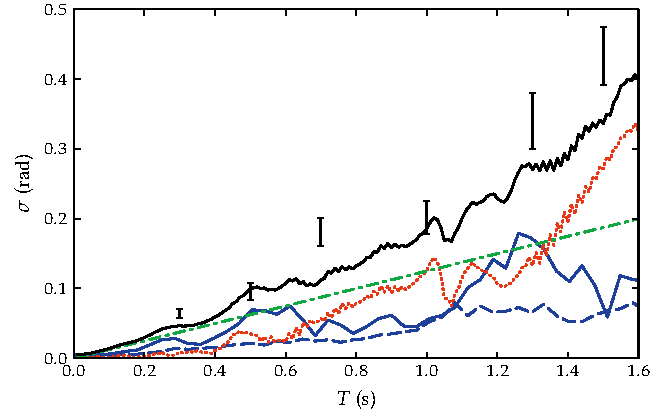
\includegraphics{figures_generated/bec_noise/echo_noise.pdf}}

    \caption{Comparison of experimental and numerically simulated interferometric contrast in the spin echo sequence.
    Plotted are the results obtained with the Wigner method (blue dashed line), Wigner method with the addition of the coupler noise (blue solid line), the noise introduced by the MW frequency instability (green dash-dotted line), the noise introduced by the imaging (red dotted line), and the combination of technical and quantum noises (black solid line), along with the experimental points (black bars).}

    \label{fig:bec-noise:phase-noise:echo-phnoise}
\end{figure}
